\PassOptionsToPackage{unicode=true}{hyperref} % options for packages loaded elsewhere
\PassOptionsToPackage{hyphens}{url}
%
\documentclass[]{book}
\usepackage{lmodern}
\usepackage{amssymb,amsmath}
\usepackage{ifxetex,ifluatex}
\usepackage{fixltx2e} % provides \textsubscript
\ifnum 0\ifxetex 1\fi\ifluatex 1\fi=0 % if pdftex
  \usepackage[T1]{fontenc}
  \usepackage[utf8]{inputenc}
  \usepackage{textcomp} % provides euro and other symbols
\else % if luatex or xelatex
  \usepackage{unicode-math}
  \defaultfontfeatures{Ligatures=TeX,Scale=MatchLowercase}
\fi
% use upquote if available, for straight quotes in verbatim environments
\IfFileExists{upquote.sty}{\usepackage{upquote}}{}
% use microtype if available
\IfFileExists{microtype.sty}{%
\usepackage[]{microtype}
\UseMicrotypeSet[protrusion]{basicmath} % disable protrusion for tt fonts
}{}
\IfFileExists{parskip.sty}{%
\usepackage{parskip}
}{% else
\setlength{\parindent}{0pt}
\setlength{\parskip}{6pt plus 2pt minus 1pt}
}
\usepackage{hyperref}
\hypersetup{
            pdftitle={Clean Air in the Time of COVID},
            pdfauthor={Ben Best, PhD},
            pdfborder={0 0 0},
            breaklinks=true}
\urlstyle{same}  % don't use monospace font for urls
\usepackage{color}
\usepackage{fancyvrb}
\newcommand{\VerbBar}{|}
\newcommand{\VERB}{\Verb[commandchars=\\\{\}]}
\DefineVerbatimEnvironment{Highlighting}{Verbatim}{commandchars=\\\{\}}
% Add ',fontsize=\small' for more characters per line
\usepackage{framed}
\definecolor{shadecolor}{RGB}{248,248,248}
\newenvironment{Shaded}{\begin{snugshade}}{\end{snugshade}}
\newcommand{\AlertTok}[1]{\textcolor[rgb]{0.94,0.16,0.16}{#1}}
\newcommand{\AnnotationTok}[1]{\textcolor[rgb]{0.56,0.35,0.01}{\textbf{\textit{#1}}}}
\newcommand{\AttributeTok}[1]{\textcolor[rgb]{0.77,0.63,0.00}{#1}}
\newcommand{\BaseNTok}[1]{\textcolor[rgb]{0.00,0.00,0.81}{#1}}
\newcommand{\BuiltInTok}[1]{#1}
\newcommand{\CharTok}[1]{\textcolor[rgb]{0.31,0.60,0.02}{#1}}
\newcommand{\CommentTok}[1]{\textcolor[rgb]{0.56,0.35,0.01}{\textit{#1}}}
\newcommand{\CommentVarTok}[1]{\textcolor[rgb]{0.56,0.35,0.01}{\textbf{\textit{#1}}}}
\newcommand{\ConstantTok}[1]{\textcolor[rgb]{0.00,0.00,0.00}{#1}}
\newcommand{\ControlFlowTok}[1]{\textcolor[rgb]{0.13,0.29,0.53}{\textbf{#1}}}
\newcommand{\DataTypeTok}[1]{\textcolor[rgb]{0.13,0.29,0.53}{#1}}
\newcommand{\DecValTok}[1]{\textcolor[rgb]{0.00,0.00,0.81}{#1}}
\newcommand{\DocumentationTok}[1]{\textcolor[rgb]{0.56,0.35,0.01}{\textbf{\textit{#1}}}}
\newcommand{\ErrorTok}[1]{\textcolor[rgb]{0.64,0.00,0.00}{\textbf{#1}}}
\newcommand{\ExtensionTok}[1]{#1}
\newcommand{\FloatTok}[1]{\textcolor[rgb]{0.00,0.00,0.81}{#1}}
\newcommand{\FunctionTok}[1]{\textcolor[rgb]{0.00,0.00,0.00}{#1}}
\newcommand{\ImportTok}[1]{#1}
\newcommand{\InformationTok}[1]{\textcolor[rgb]{0.56,0.35,0.01}{\textbf{\textit{#1}}}}
\newcommand{\KeywordTok}[1]{\textcolor[rgb]{0.13,0.29,0.53}{\textbf{#1}}}
\newcommand{\NormalTok}[1]{#1}
\newcommand{\OperatorTok}[1]{\textcolor[rgb]{0.81,0.36,0.00}{\textbf{#1}}}
\newcommand{\OtherTok}[1]{\textcolor[rgb]{0.56,0.35,0.01}{#1}}
\newcommand{\PreprocessorTok}[1]{\textcolor[rgb]{0.56,0.35,0.01}{\textit{#1}}}
\newcommand{\RegionMarkerTok}[1]{#1}
\newcommand{\SpecialCharTok}[1]{\textcolor[rgb]{0.00,0.00,0.00}{#1}}
\newcommand{\SpecialStringTok}[1]{\textcolor[rgb]{0.31,0.60,0.02}{#1}}
\newcommand{\StringTok}[1]{\textcolor[rgb]{0.31,0.60,0.02}{#1}}
\newcommand{\VariableTok}[1]{\textcolor[rgb]{0.00,0.00,0.00}{#1}}
\newcommand{\VerbatimStringTok}[1]{\textcolor[rgb]{0.31,0.60,0.02}{#1}}
\newcommand{\WarningTok}[1]{\textcolor[rgb]{0.56,0.35,0.01}{\textbf{\textit{#1}}}}
\usepackage{longtable,booktabs}
% Fix footnotes in tables (requires footnote package)
\IfFileExists{footnote.sty}{\usepackage{footnote}\makesavenoteenv{longtable}}{}
\usepackage{graphicx,grffile}
\makeatletter
\def\maxwidth{\ifdim\Gin@nat@width>\linewidth\linewidth\else\Gin@nat@width\fi}
\def\maxheight{\ifdim\Gin@nat@height>\textheight\textheight\else\Gin@nat@height\fi}
\makeatother
% Scale images if necessary, so that they will not overflow the page
% margins by default, and it is still possible to overwrite the defaults
% using explicit options in \includegraphics[width, height, ...]{}
\setkeys{Gin}{width=\maxwidth,height=\maxheight,keepaspectratio}
\setlength{\emergencystretch}{3em}  % prevent overfull lines
\providecommand{\tightlist}{%
  \setlength{\itemsep}{0pt}\setlength{\parskip}{0pt}}
\setcounter{secnumdepth}{5}
% Redefines (sub)paragraphs to behave more like sections
\ifx\paragraph\undefined\else
\let\oldparagraph\paragraph
\renewcommand{\paragraph}[1]{\oldparagraph{#1}\mbox{}}
\fi
\ifx\subparagraph\undefined\else
\let\oldsubparagraph\subparagraph
\renewcommand{\subparagraph}[1]{\oldsubparagraph{#1}\mbox{}}
\fi

% set default figure placement to htbp
\makeatletter
\def\fps@figure{htbp}
\makeatother

\usepackage{booktabs}
\usepackage{amsthm}
\makeatletter
\def\thm@space@setup{%
  \thm@preskip=8pt plus 2pt minus 4pt
  \thm@postskip=\thm@preskip
}
\makeatother
\usepackage{etoolbox}
\makeatletter
\providecommand{\subtitle}[1]{% add subtitle to \maketitle
  \apptocmd{\@title}{\par {\large #1 \par}}{}{}
}
\makeatother
\usepackage[]{natbib}
\bibliographystyle{apalike}

\title{Clean Air in the Time of COVID}
\providecommand{\subtitle}[1]{}
\subtitle{Use Cases for Google Earth Engine \& Sentiment Analysis}
\author{Ben Best, PhD}
\date{2020-05-26}

\begin{document}
\maketitle

{
\setcounter{tocdepth}{1}
\tableofcontents
}
\hypertarget{overview}{%
\chapter*{Overview}\label{overview}}
\addcontentsline{toc}{chapter}{Overview}

These materials are for a 45 minute teaching demonstration on 2020-05-26 oriented towards students in the new Masters in Environmental Data Science at UCSB.

\hypertarget{motivation}{%
\section*{Motivation}\label{motivation}}
\addcontentsline{toc}{section}{Motivation}

This is an exciting time for the emerging field of Environmental Data Science. Environmental problems are increasingly complex and require advanced technical skills to translate the ever expanding flow of data into actionable insights.

\hypertarget{technologies}{%
\subsection*{Technologies}\label{technologies}}
\addcontentsline{toc}{subsection}{Technologies}

The two specific technologies featured in this teaching demonstration highlight some of the most promising aspects of truly :

\begin{itemize}
\item
  \textbf{Google Earth Engine} leverages the massive storage and computational capabilities of the Google Cloud to analyze petabytes of the publicly available satellite data. For instance, global climatologies averaging across 40 years of temperature can be calculated and mapped in seconds. This is a truly \emph{big data} platform!
\item
  \textbf{TensorFlow} is the machine learning software made open-source by Google. It is the most commonly used software for audio, text and image analysis. More specifically tensorflow allows construction of \emph{convolutional neural networks}, which represent a layering of nodes to enable complex pattern matching. These \emph{deep learning} models have been popularized by their ability to beat the best human at the most complex game of Go, self-drive vehicles, Netflix recommendations, Spotify playlists and respond to your beck and call through Alexa's voice commands.
\end{itemize}

\hypertarget{motivating-use-case}{%
\subsection*{Motivating Use Case}\label{motivating-use-case}}
\addcontentsline{toc}{subsection}{Motivating Use Case}

For the first time in decades, Mount Everest was visible from Kathmandu due to improved air quality.

--- Tom Patterson (@MtnMapper) May 21, 2020

The positive effect of the Lockdown in India's environment can be seen in New Delhi.This picture depicts the air quality of New Delhi before \& after Lockdown.Source - https://t.co/VoG0UbpFzE

--- GurumaujSatsangi (@GurumaujS) April 23, 2020

\hypertarget{prerequisites}{%
\section*{Prerequisites}\label{prerequisites}}
\addcontentsline{toc}{section}{Prerequisites}

See the Setup for required software. For this demonstration to make the most sense, it's preferable that you're familiar with:

\begin{itemize}
\tightlist
\item
  \textbf{R}
\item
  \textbf{GIS}
\end{itemize}

\hypertarget{setup}{%
\chapter*{Setup}\label{setup}}
\addcontentsline{toc}{chapter}{Setup}

\hypertarget{apply-for-accounts}{%
\section{Apply for accounts}\label{apply-for-accounts}}

\hypertarget{google-earth-engine-gee-account}{%
\subsection{Google Earth Engine (GEE) account}\label{google-earth-engine-gee-account}}

Please visit:

\begin{itemize}
\tightlist
\item
  \href{https://signup.earthengine.google.com/\#!/}{Google Earth Engine signup}
\end{itemize}

You may need to log out and back into your web browser as the preferred Google account to request permissions. This approval process can take days to weeks unfortunately.

\hypertarget{twitter-developer-account}{%
\subsection{Twitter developer account}\label{twitter-developer-account}}

Please visit:

\begin{itemize}
\tightlist
\item
  \href{https://developer.twitter.com/en/apply-for-access}{Twitter developer signup}
\end{itemize}

I recieved an email for clarification and had the account approved and running by the end of the day.

\hypertarget{install-software}{%
\section{Install software}\label{install-software}}

This workshop will require the following software installed on your machine:

\begin{itemize}
\tightlist
\item
  \href{http://cran.cnr.berkeley.edu/}{R}
\item
  \href{https://www.rstudio.com/products/rstudio/download/\#download}{RStudio}
\end{itemize}

Please download the appropriate stable release for your operating system.

\hypertarget{launch-rstudio}{%
\section{Launch RStudio}\label{launch-rstudio}}

RStudio is an integrated development environment (IDE) for editing text in the code editor, running commands in the R console, viewing defined objects in the workspace and past commands in the history, and viewing plots, files and help. Here's a layout of the panes in RStudio, each of which can have several tabs for alternate functionality:

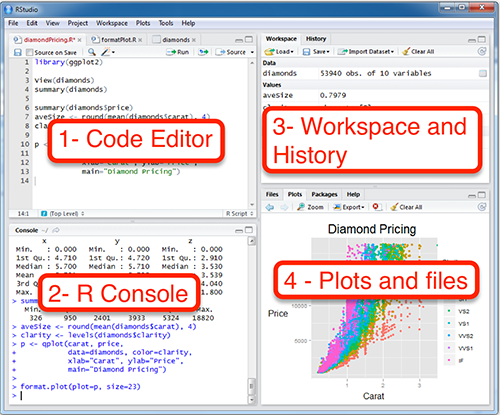
\includegraphics{images/rstudio.png}

Check out the Help \textgreater{} Cheatsheets \textgreater{} \href{https://github.com/rstudio/cheatsheets/raw/master/rstudio-ide.pdf}{RStudio IDE Cheat Sheet}.

\hypertarget{fork-and-clone-the-github-repository}{%
\section{Fork and Clone the Github Repository}\label{fork-and-clone-the-github-repository}}

Please visit \url{https://github.com/bbest/meds-demo}, signed into Github. Then into your own writable user space.

Here is the Github repository of the source files for this demonstration:

\url{https://github.com/bbest/meds-demo}

You are encouraged to \href{https://help.github.com/en/github/getting-started-with-github/fork-a-repo}{fork the repo in Github} and \href{https://happygitwithr.com/rstudio-git-github.html\#clone-the-new-github-repository-to-your-computer-via-rstudio}{clone it in RStudio}.

Then you can follow along in RStudio by evaluating the chunks of R code, while referencing the website:

\url{http://benbestphd.com/meds-demo}

\hypertarget{install-r-packages}{%
\section{Install R Packages}\label{install-r-packages}}

Here's a bit of code to install packages that we'll use throughout the workshop. Please copy and paste this code into your console.

\begin{Shaded}
\begin{Highlighting}[]
\CommentTok{# use librarian to load libraries, installing if needed}
\ControlFlowTok{if}\NormalTok{ (}\OperatorTok{!}\KeywordTok{require}\NormalTok{(}\StringTok{"librarian"}\NormalTok{)) }\KeywordTok{install.packages}\NormalTok{(}\StringTok{"librarian"}\NormalTok{)}
\KeywordTok{library}\NormalTok{(}\StringTok{"librarian"}\NormalTok{)}

\CommentTok{# load packages}
\NormalTok{pkgs <-}\StringTok{ }\KeywordTok{c}\NormalTok{(}
  \CommentTok{# general}
  \StringTok{"tidyverse"}\NormalTok{,}\StringTok{"jsonlite"}\NormalTok{,}\StringTok{"glue"}\NormalTok{,}\StringTok{"here"}\NormalTok{,}\StringTok{"units"}\NormalTok{,}

  \CommentTok{# satellite}
  \StringTok{"sf"}\NormalTok{,}
  
  \CommentTok{# sentiment}
  \StringTok{"rtweet"}\NormalTok{,}\StringTok{"tidytext"}\NormalTok{)}
\KeywordTok{shelf}\NormalTok{(pkgs)}

\CommentTok{# report on versions of software & packages}
\KeywordTok{sessionInfo}\NormalTok{()}
\end{Highlighting}
\end{Shaded}

\begin{verbatim}
## R version 3.5.2 (2018-12-20)
## Platform: x86_64-apple-darwin15.6.0 (64-bit)
## Running under: macOS Mojave 10.14.6
## 
## Matrix products: default
## BLAS: /Library/Frameworks/R.framework/Versions/3.5/Resources/lib/libRblas.0.dylib
## LAPACK: /Library/Frameworks/R.framework/Versions/3.5/Resources/lib/libRlapack.dylib
## 
## locale:
## [1] en_US.UTF-8/en_US.UTF-8/en_US.UTF-8/C/en_US.UTF-8/en_US.UTF-8
## 
## attached base packages:
## [1] stats     graphics  grDevices utils     datasets  methods   base     
## 
## other attached packages:
##  [1] tidytext_0.2.2  rtweet_0.7.0    sf_0.8-0        units_0.6-6    
##  [5] here_0.1        glue_1.4.1      jsonlite_1.6.1  forcats_0.4.0  
##  [9] stringr_1.4.0   dplyr_0.8.5     purrr_0.3.4     readr_1.3.1    
## [13] tidyr_1.1.0     tibble_3.0.1    ggplot2_3.3.0   tidyverse_1.3.0
## [17] librarian_1.7.0
## 
## loaded via a namespace (and not attached):
##  [1] Rcpp_1.0.4.6       lubridate_1.7.8    lattice_0.20-38    class_7.3-15      
##  [5] assertthat_0.2.1   rprojroot_1.3-2    digest_0.6.25      R6_2.4.1          
##  [9] cellranger_1.1.0   backports_1.1.7    reprex_0.3.0       evaluate_0.14     
## [13] e1071_1.7-3        httr_1.4.1         pillar_1.4.4       rlang_0.4.6       
## [17] readxl_1.3.1       rstudioapi_0.11    Matrix_1.2-18      rmarkdown_2.1     
## [21] munsell_0.5.0      broom_0.5.5        janeaustenr_0.1.5  compiler_3.5.2    
## [25] modelr_0.1.5       xfun_0.14          pkgconfig_2.0.3    vembedr_0.1.3     
## [29] htmltools_0.4.0    tidyselect_1.1.0   bookdown_0.16      fansi_0.4.1       
## [33] crayon_1.3.4       dbplyr_1.4.2       withr_2.2.0        SnowballC_0.6.0   
## [37] grid_3.5.2         nlme_3.1-142       gtable_0.3.0       lifecycle_0.2.0   
## [41] DBI_1.1.0          magrittr_1.5       tokenizers_0.2.1   scales_1.1.1      
## [45] KernSmooth_2.23-16 cli_2.0.2          stringi_1.4.6      fs_1.3.1          
## [49] xml2_1.2.2         ellipsis_0.3.1     generics_0.0.2     vctrs_0.3.0       
## [53] tools_3.5.2        hms_0.5.3          yaml_2.2.1         colorspace_1.4-1  
## [57] classInt_0.4-3     rvest_0.3.5        knitr_1.28         haven_2.2.0
\end{verbatim}

\hypertarget{create-rmarkdown-file}{%
\section{Create Rmarkdown file}\label{create-rmarkdown-file}}

Rmarkdown is a dynamic document format that allows you to knit chunks of R code with formatted text (aka markdown). We recommend that you use this format for keeping a reproducible research document as you work through the lessons To get started, File \textgreater{} New File \textgreater{} Rmarkdown\ldots{} and go with default HTML document and give any title you like (default ``Untitled'' or ``test'' or ``First Rmd'' is fine).

Check out the Help \textgreater{} Markdown Quick Reference and Help \textgreater{} Cheatsheets \textgreater{} \href{https://github.com/rstudio/cheatsheets/raw/master/rmarkdown-2.0.pdf}{R Markdown Cheat Sheet}.

Here's a 1 minute video on the awesomeness of Rmarkdown:

\hypertarget{satellite}{%
\chapter{Satellite}\label{satellite}}

\hypertarget{objectives}{%
\section*{Objectives}\label{objectives}}
\addcontentsline{toc}{section}{Objectives}

\hypertarget{question}{%
\subsection*{Question}\label{question}}
\addcontentsline{toc}{subsection}{Question}

\begin{itemize}
\tightlist
\item
  How have emissions related to air quality changed since COVID-19 lockdowns were put in place?
\end{itemize}

\hypertarget{study-area-delhi-india}{%
\subsection*{Study area: Delhi, India}\label{study-area-delhi-india}}
\addcontentsline{toc}{subsection}{Study area: Delhi, India}

\begin{itemize}
\tightlist
\item
  We'll use \textbf{Delhi, India} as our initial city study area. Prime Minister Modhi issued a nationwide lockdown on 24 March, 2020.
\end{itemize}

\textbf{News}:

\begin{itemize}
\tightlist
\item
  \href{https://www.cnn.com/2020/04/22/world/air-pollution-reduction-cities-coronavirus-intl-hnk/index.html}{Air pollution falls by unprecedented levels in major global cities during coronavirus lockdowns - CNN}
\item
  \href{https://www.cnn.com/2020/04/23/india/india-air-pollution-coronavirus-nasa-intl/index.html}{India: air pollution in the north has hit a 20-year low, NASA report says - CNN}
\item
  \href{https://smartairfilters.com/en/blog/delhi-pm25-air-pollution-decrease-coronavirus/}{Fact Check: Is The COVID-19 Lockdown Decreasing Delhi Air Pollution? - Smart Air Filters}
\end{itemize}

\hypertarget{learning-outcomes}{%
\subsection*{Learning outcomes}\label{learning-outcomes}}
\addcontentsline{toc}{subsection}{Learning outcomes}

The student will learn how to:

\begin{enumerate}
\def\labelenumi{\arabic{enumi}.}
\tightlist
\item
  Browse Google Earth Engine's data catalogue
\item
  Examine basic information about the dataset
\item
  Map datasets in the Code Editor
\item
  Upload assets, such as a polygon
\item
  Adjust time period for averaging
\item
  Generate a time series chart for satellite data extracted to a region
\item
  Download data as a text file (csv)
\end{enumerate}

\hypertarget{prerequisites-1}{%
\section*{Prerequisites}\label{prerequisites-1}}
\addcontentsline{toc}{section}{Prerequisites}

A \textbf{Google Earth Engine account} that is associated with a Google account, such as from Gmail, is required to log into \url{https://code.earthengine.google.com}.

If you need a GEE account, please visit \url{https://signup.earthengine.google.com}.

You may need to log out and back into your web browser as the preferred Google account to request permissions. This approval process can take days to weeks unfortunately.

\hypertarget{get-city-boundary}{%
\section{Get city boundary}\label{get-city-boundary}}

The first step is to define our study area. I made a little R helper function \texttt{city2zip()} to:

\begin{enumerate}
\def\labelenumi{\arabic{enumi}.}
\tightlist
\item
  Fetch the administrative boundary from the \href{https://nominatim.org/release-docs/develop/api/Search/}{Nominatim OpenStreetMap API} given a city name.
\item
  Extract the polygon information, convert to shapefile and zip for upload into GEE.
\end{enumerate}

\begin{Shaded}
\begin{Highlighting}[]
\KeywordTok{source}\NormalTok{(}\StringTok{"functions.R"}\NormalTok{)}

\KeywordTok{city2zip}\NormalTok{(}\StringTok{"Delhi, India"}\NormalTok{)}
\end{Highlighting}
\end{Shaded}

The function returns the paths to files generated. You will use this zip file to upload into GEE as an asset.

\hypertarget{browse-datasets-tag-no2}{%
\section{Browse datasets, tag no2}\label{browse-datasets-tag-no2}}

Visit \url{https://earthengine.google.com} \textgreater{} Datasets (upper right). Be sure to explore the many datasets available here.

Since we know we want Nitrogen Dioxide (NO\textsubscript{2}), click on Browse by tags and Filter by ``no2''. You should see two datasets:

\begin{figure}
\centering
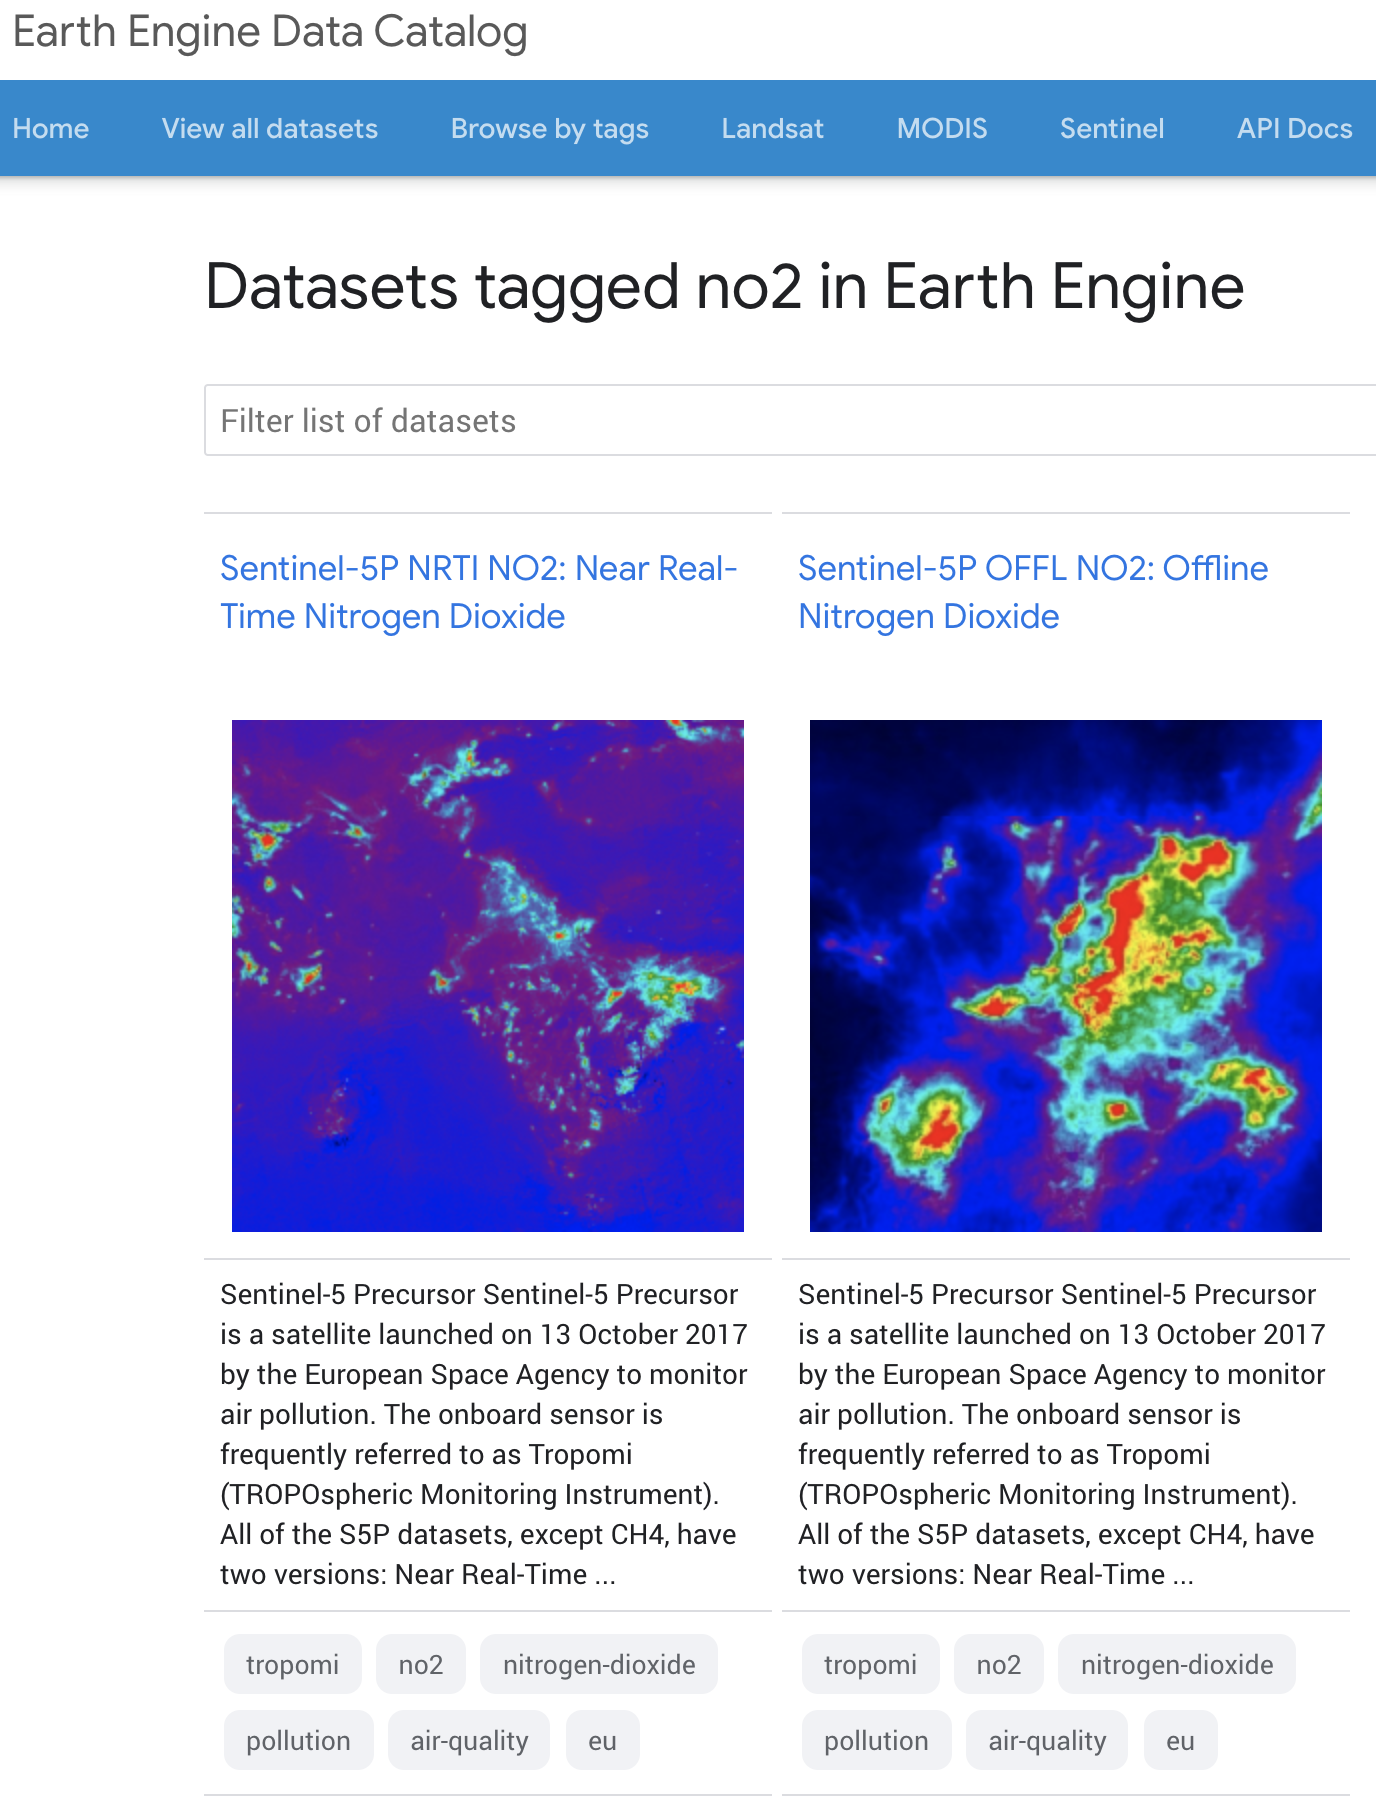
\includegraphics{images/gee_datasets-tag-no2.png}
\caption{Screenshot of GEE data catalog filtered by tag ``no2'' showing two datasets.}
\end{figure}

\hypertarget{view-dataset-info}{%
\section{View dataset info}\label{view-dataset-info}}

Please click on ``Sentinel-5P NRTI NO2: Near Real-Time Nitrogen Dioxide'' to get the dataset view. Explore the metadata for this dataset.

\hypertarget{questions}{%
\section{Questions}\label{questions}}

\begin{enumerate}
\def\labelenumi{\arabic{enumi}.}
\tightlist
\item
  How many years of data are available?
\item
  How does this compare with the other ``Offline'' dataset?
\item
  Which of the bands do we want to use that is closest to the surface?
\item
  What are the units of the band ``NO2\_column\_number\_density''?
\item
  What is its maximum value?
\end{enumerate}

\hypertarget{answers}{%
\subsection{Answers}\label{answers}}

\begin{enumerate}
\def\labelenumi{\arabic{enumi}.}
\tightlist
\item
  2018-07-10 - Present, so \textasciitilde{}1.5 months shy of 2 years
\item
  2018-06-28 - Present, so only \textasciitilde{} 0.5 month longer
\item
  mol/m\textsuperscript{2}
\item
  0.0096
\end{enumerate}

\hypertarget{launch-code-editor-with-dataset}{%
\section{Launch Code Editor with dataset}\label{launch-code-editor-with-dataset}}

Scroll to the bottom. You should see the following snippet of JavaScript code:

\begin{Shaded}
\begin{Highlighting}[]
\KeywordTok{var}\NormalTok{ collection }\OperatorTok{=} \VariableTok{ee}\NormalTok{.}\AttributeTok{ImageCollection}\NormalTok{(}\StringTok{'COPERNICUS/S5P/NRTI/L3_NO2'}\NormalTok{)}
\NormalTok{  .}\AttributeTok{select}\NormalTok{(}\StringTok{'NO2_column_number_density'}\NormalTok{)}
\NormalTok{  .}\AttributeTok{filterDate}\NormalTok{(}\StringTok{'2019-06-01'}\OperatorTok{,} \StringTok{'2019-06-06'}\NormalTok{)}\OperatorTok{;}

\KeywordTok{var}\NormalTok{ band_viz }\OperatorTok{=} \OperatorTok{\{}
  \DataTypeTok{min}\OperatorTok{:} \DecValTok{0}\OperatorTok{,}
  \DataTypeTok{max}\OperatorTok{:} \FloatTok{0.0002}\OperatorTok{,}
  \DataTypeTok{palette}\OperatorTok{:}\NormalTok{ [}\StringTok{'black'}\OperatorTok{,} \StringTok{'blue'}\OperatorTok{,} \StringTok{'purple'}\OperatorTok{,} \StringTok{'cyan'}\OperatorTok{,} \StringTok{'green'}\OperatorTok{,} \StringTok{'yellow'}\OperatorTok{,} \StringTok{'red'}\NormalTok{]}
\OperatorTok{\};}

\VariableTok{Map}\NormalTok{.}\AttributeTok{addLayer}\NormalTok{(}\VariableTok{collection}\NormalTok{.}\AttributeTok{mean}\NormalTok{()}\OperatorTok{,}\NormalTok{ band_viz}\OperatorTok{,} \StringTok{'S5P N02'}\NormalTok{)}\OperatorTok{;}
\VariableTok{Map}\NormalTok{.}\AttributeTok{setCenter}\NormalTok{(}\FloatTok{65.27}\OperatorTok{,} \FloatTok{24.11}\OperatorTok{,} \DecValTok{4}\NormalTok{)}\OperatorTok{;}
\end{Highlighting}
\end{Shaded}

Click the button at the bottom to launch the Code Editor with this dataset loading JavaScript code:

Open in Code Editor

\hypertarget{run-the-initial-dataset-script}{%
\section{Run the initial dataset script}\label{run-the-initial-dataset-script}}

You should now be seeing the Code Editor. Here are some labels for the user interface to orient yourself:

!{[}Credit: \href{images/gee_02_codeeditor.png}{Google Earth Engine: Code Editor}

Click \textbf{Run} to run the script. Voila! You should see tiles of the satellite data layer appear in the lower Map pane:

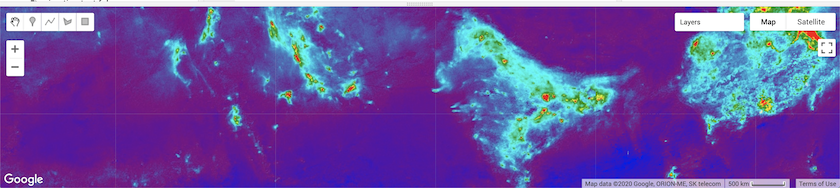
\includegraphics{images/gee_run-init-dataset.png}

Be sure to try out the zoom (+/-) and pan (hand icon) to move around.

\hypertarget{modify-the-script-so-satellite-layer-is-semi-transparent}{%
\section{Modify the script so satellite layer is semi-transparent}\label{modify-the-script-so-satellite-layer-is-semi-transparent}}

Decrease the ``opacity'' (Search for this word under Docs tab; see documentation for Map.addLayer then ee.data.getMapId) in and add the \texttt{opacity} parameter with a value of \texttt{0.5} to the \texttt{band\_viz} definition like so (don't forget the extra comma):

\begin{Shaded}
\begin{Highlighting}[]
\KeywordTok{var}\NormalTok{ band_viz }\OperatorTok{=} \OperatorTok{\{}
  \DataTypeTok{min}\OperatorTok{:} \DecValTok{0}\OperatorTok{,}
  \DataTypeTok{max}\OperatorTok{:} \FloatTok{0.0002}\OperatorTok{,}
  \DataTypeTok{palette}\OperatorTok{:}\NormalTok{ [}\StringTok{'black'}\OperatorTok{,} \StringTok{'blue'}\OperatorTok{,} \StringTok{'purple'}\OperatorTok{,} \StringTok{'cyan'}\OperatorTok{,} \StringTok{'green'}\OperatorTok{,} \StringTok{'yellow'}\OperatorTok{,} \StringTok{'red'}\NormalTok{]}\OperatorTok{,}
  \DataTypeTok{opacity}\OperatorTok{:} \FloatTok{0.5}
\OperatorTok{\};}
\end{Highlighting}
\end{Shaded}

Save the file and Run. I am choosing to save this file as ``no2'' under the ``meds-demo'' repository in the Script manager pane (upper left).

\hypertarget{add-city-polygon-asset}{%
\section{Add city polygon asset}\label{add-city-polygon-asset}}

Use the Asset Manager (Assets tab in upper left) to now add your study area by Uploading a {NEW} Shape file. Drag \texttt{city\_Delhi.India.zip} in your file system to the {SELECT} button. Click {UPLOAD} to start upload.

Now click the Tasks tab (upper right) to see that this process is initiated, but not yet complete (spinny gear on right). It should complete within a minute. You might need to refresh your browser for the asset to appear.

Hover over the newly added asset city\_Delhi-India in your Assets pane and click on the blue right arrow to import it into your script.

For more on this topic, see \href{https://developers.google.com/earth-engine/asset_manager}{Managing Assets}.

\hypertarget{add-to-city-to-map}{%
\section{Add to city to map}\label{add-to-city-to-map}}

Notice how it brings in the asset as a default variable named \texttt{table}. I suggest changing the name of this variable to something friendlier like \texttt{city\_ply}, short for city polygon.

Now center the map on this polygon (vs \texttt{Map.setCenter(65.27,\ 24.11,\ 4);}) and add it as a layer to be drawn on the map:

\begin{Shaded}
\begin{Highlighting}[]
\VariableTok{Map}\NormalTok{.}\AttributeTok{addLayer}\NormalTok{(}\VariableTok{collection}\NormalTok{.}\AttributeTok{mean}\NormalTok{()}\OperatorTok{,}\NormalTok{ band_viz}\OperatorTok{,} \StringTok{'S5P N02'}\NormalTok{)}\OperatorTok{;}
\VariableTok{Map}\NormalTok{.}\AttributeTok{centerObject}\NormalTok{(city_ply)}\OperatorTok{;}
\VariableTok{Map}\NormalTok{.}\AttributeTok{addLayer}\NormalTok{(city_ply}\OperatorTok{,} \OperatorTok{\{}\DataTypeTok{color}\OperatorTok{:} \StringTok{'black'}\OperatorTok{\},} \StringTok{'Delhi'}\NormalTok{)}\OperatorTok{;}
\end{Highlighting}
\end{Shaded}

For more, see:

\begin{itemize}
\tightlist
\item
  \href{https://developers.google.com/earth-engine/geometry_visualization_info}{Geometry Visualization and Information}
\end{itemize}

\hypertarget{create-time-series-chart}{%
\section{Create time series chart}\label{create-time-series-chart}}

Next let's generate a \href{https://developers.google.com/earth-engine/charts_image_series}{Time Series Chart}, which is available as user interface (\texttt{ui}) that we can print (vs embedding in a dedicate \href{https://developers.google.com/earth-engine/apps}{app} or \href{https://developers.google.com/earth-engine/ui}{user interface} -- for another day).

Its two required parameters are for an image collection and a region (find parameters in the Docs). The third parameter is for the reducer, which is the function that reduces the many pixels into a single value. In our case we want to take the average so we'll use the \texttt{ee.Reducer.mean()} function.

\begin{Shaded}
\begin{Highlighting}[]
\AttributeTok{print}\NormalTok{(}\VariableTok{ui}\NormalTok{.}\VariableTok{Chart}\NormalTok{.}\VariableTok{image}\NormalTok{.}\AttributeTok{series}\NormalTok{(}
\NormalTok{  collection}\OperatorTok{,} 
\NormalTok{  city_ply}\OperatorTok{,} 
  \VariableTok{ee}\NormalTok{.}\VariableTok{Reducer}\NormalTok{.}\AttributeTok{mean}\NormalTok{()))}\OperatorTok{;}
\end{Highlighting}
\end{Shaded}

Save and Run. Yay! You should see a time series chart in the Console:

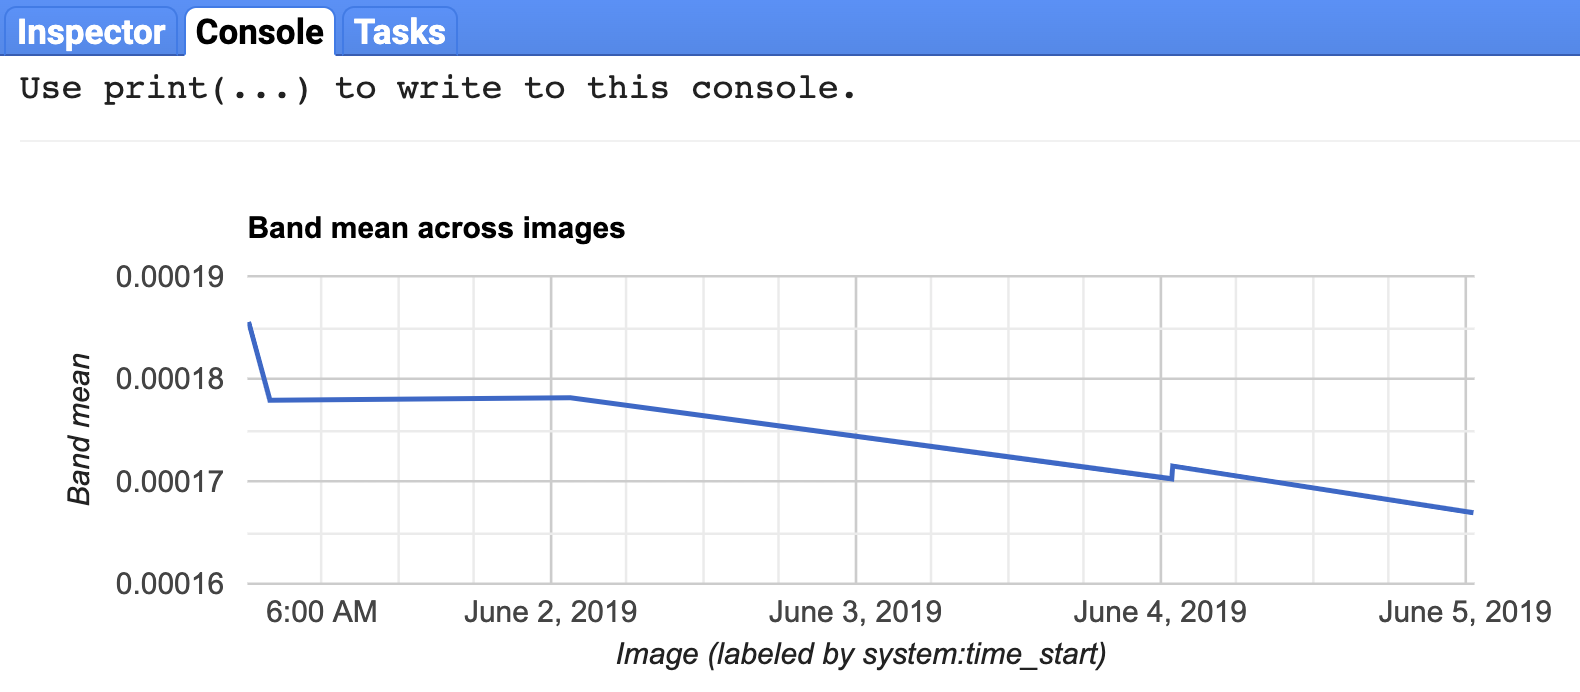
\includegraphics{images/gee_ts-chart_1-week.png}

\hypertarget{expand-dates-to-all-available}{%
\section{Expand dates to all available}\label{expand-dates-to-all-available}}

But that was only for the default week of `2019-06-01' to `2019-06-06' and we know this dataset is available for a longer period. Let's update \texttt{.filterDate()} to use the entire range of available data in line 3:

\begin{Shaded}
\begin{Highlighting}[]
\NormalTok{  .}\AttributeTok{filterDate}\NormalTok{(}\StringTok{'2018-07-10'}\OperatorTok{,} \StringTok{'2020-05-26'}\NormalTok{)}\OperatorTok{;}
\end{Highlighting}
\end{Shaded}

Save and Run again. It should take a bit longer to process, since it's now extracting almost 2 years worth of data in the city polygon. Once the plot shows up in the Console again, click the upper right arrow to pop it into its own dedicated window.

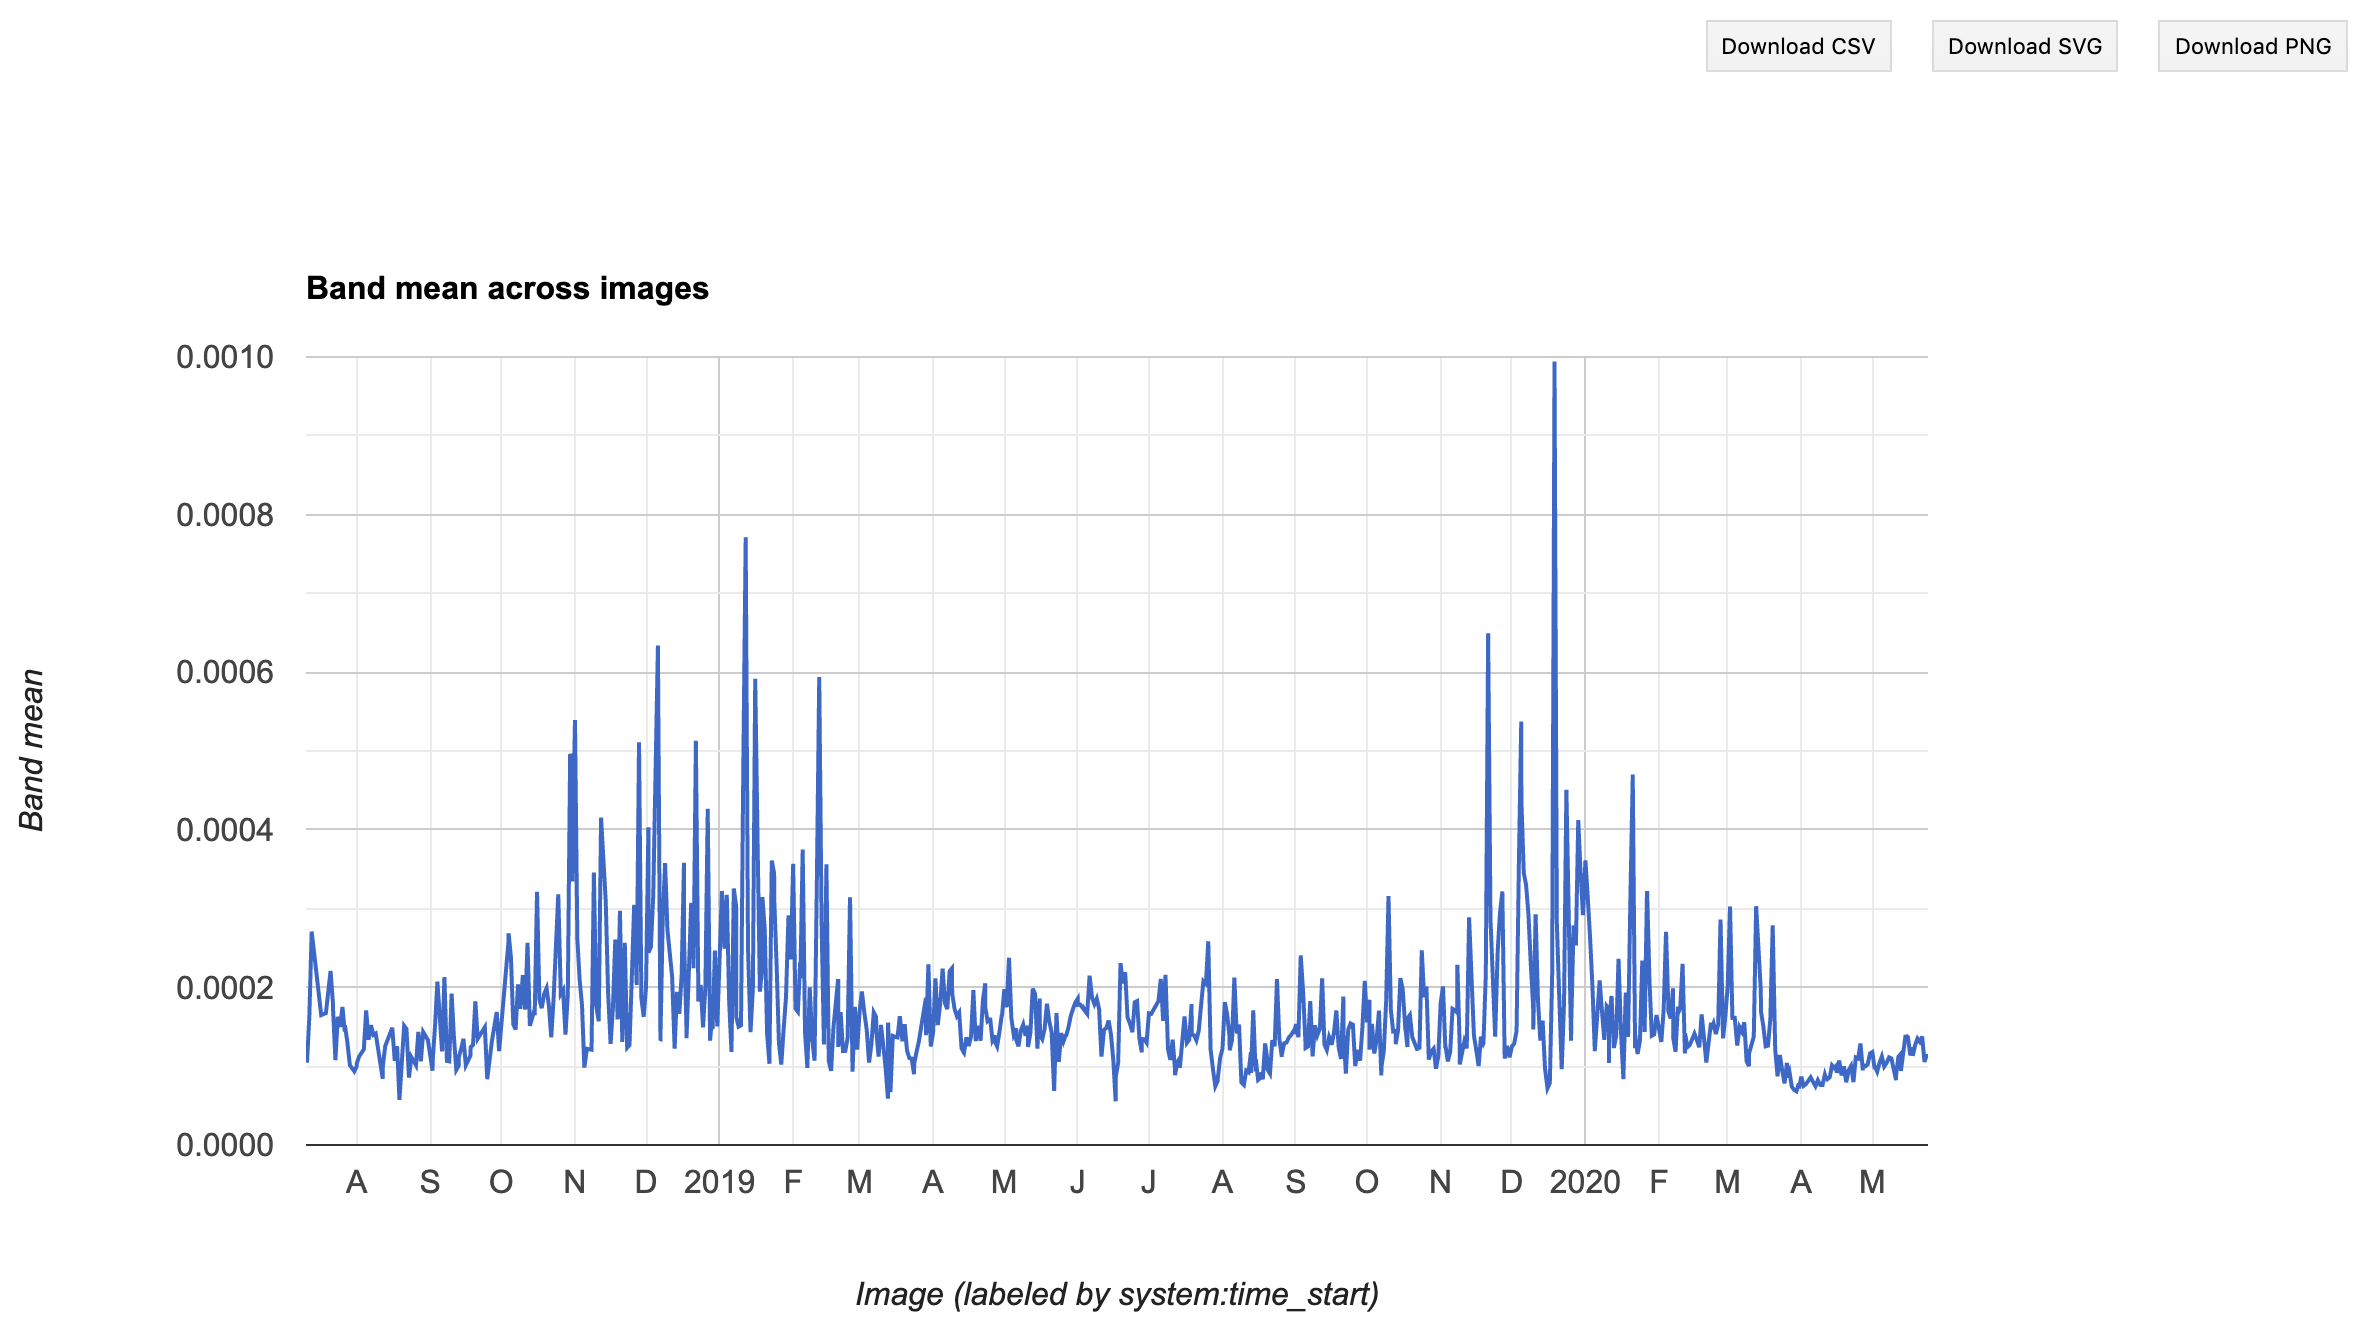
\includegraphics{images/gee_ts-chart_all-popout.png}

\hypertarget{download-csv}{%
\section{Download CSV}\label{download-csv}}

In the popped out window of the time series chart, download the comma-seperated value (CSV) text file by clicking the {Download CSV} button. I save my file into \texttt{data/no2\_gee\_Delhi-India.csv} of this Github repository.

\hypertarget{conclusions}{%
\section*{Conclusions}\label{conclusions}}
\addcontentsline{toc}{section}{Conclusions}

It is similarly creating an average raster for the entire time domain of this dataset in the Map pane. Try zooming out, realizing that is happening globally. Now that's big data! In a tiny amount of time, with minor effort.

\hypertarget{your-turn}{%
\section{Your Turn}\label{your-turn}}

\begin{itemize}
\tightlist
\item
  Pick another city and start from the top. Generate a polygon zip, upload as an asset and generate the time series.
\end{itemize}

\hypertarget{further-resources}{%
\section*{Further Resources}\label{further-resources}}
\addcontentsline{toc}{section}{Further Resources}

\hypertarget{google-earth-engine}{%
\subsection*{Google Earth Engine}\label{google-earth-engine}}
\addcontentsline{toc}{subsection}{Google Earth Engine}

\begin{itemize}
\tightlist
\item
  \href{https://geohackweek.github.io/GoogleEarthEngine/}{GEE Lessons - GeoHackWeek}: Software Carpentry style
\item
  \href{https://r-spatial.github.io/rgee/}{rgee}: R package for GEE; still in early development
\item
  \citep{gorelickGoogleEarthEngine2017a}
\end{itemize}

\hypertarget{sentiment}{%
\chapter{Sentiment}\label{sentiment}}

\hypertarget{objectives-1}{%
\section*{Objectives}\label{objectives-1}}
\addcontentsline{toc}{section}{Objectives}

\hypertarget{question-1}{%
\subsection*{Question}\label{question-1}}
\addcontentsline{toc}{subsection}{Question}

\begin{itemize}
\tightlist
\item
  How has sentiment around air quality and clean energy changed since air became cleaner?
\end{itemize}

\hypertarget{motivation-1}{%
\subsection*{Motivation}\label{motivation-1}}
\addcontentsline{toc}{subsection}{Motivation}

Sentiment can be evaluated as either positive or negative. This \textbf{binary classification} is the most basic response for \textbf{machine learning}, thus a good example for a lesson on machine learning. Text however can have many complicated forms, such as negating terms (eg ``happy'' vs ``\emph{\textbf{not}} happy''), which makes it a good candidate for \textbf{deep learning}.

\hypertarget{approach}{%
\subsection*{Approach}\label{approach}}
\addcontentsline{toc}{subsection}{Approach}

\begin{enumerate}
\def\labelenumi{\arabic{enumi}.}
\tightlist
\item
  Get a set of sample tweets before and after the lockdown with some of key terms.
\item
  Lookup tweeted words with dictionaries labelling positive or negative, and tally the score. Bren's own Casey O'Hara \& Jessica Couture already explained this approach well in their Eco-Data-Science workshop \href{https://github.com/oharac/text_workshop}{Text analysis with R} (2019-02-05).
\item
  Introduce TensorFlow starting with a pre-trained model.
\item
  Use a sample of the Sentiment140 twitter dataset to train an existing natural language processing (NLP) model.
\item
  Predict that over time.
\end{enumerate}

\hypertarget{prerequisites-2}{%
\section*{Prerequisites}\label{prerequisites-2}}
\addcontentsline{toc}{section}{Prerequisites}

A \textbf{Twitter developer account} is required to download tweets and access the \url{https://developer.twitter.com/en/dashboard}. You'll need to apply via the \href{https://developer.twitter.com/en/apply-for-access}{Twitter developer signup}.

I recieved an email for clarification and had the account approved and running by the end of the day.

\hypertarget{setup-twitter-token}{%
\section{Setup Twitter token}\label{setup-twitter-token}}

We'll use the \href{https://rtweet.info}{rtweet} R package to get twitter data. You'll need to setup an access token though after applying for a Twitter API

See \href{https://rtweet.info/articles/auth.html}{Obtaining and using access tokens • rtweet}:

\begin{itemize}
\item
  Creating a Twitter App
\item
  Authorization methods

  \begin{itemize}
  \item
    \begin{enumerate}
    \def\labelenumi{\arabic{enumi}.}
    \setcounter{enumi}{1}
    \tightlist
    \item
      Access token/secret method
    \end{enumerate}
  \end{itemize}
\item
  Authorization in future R sessions

\begin{Shaded}
\begin{Highlighting}[]
\KeywordTok{library}\NormalTok{(rtweet)}
\KeywordTok{get_token}\NormalTok{()}
\end{Highlighting}
\end{Shaded}
\end{itemize}

For \texttt{search\_fullarchive} also tried to setup \href{https://developer.twitter.com/en/account/environments}{Dev environment --- Twitter Developers}, but that didn't seem to work.

\hypertarget{load-r-packages}{%
\section{Load R packages}\label{load-r-packages}}

\begin{Shaded}
\begin{Highlighting}[]
\CommentTok{# load libraries ----}
\CommentTok{# use librarian to load libraries, installing if needed}
\ControlFlowTok{if}\NormalTok{ (}\OperatorTok{!}\KeywordTok{require}\NormalTok{(}\StringTok{"librarian"}\NormalTok{)) }\KeywordTok{install.packages}\NormalTok{(}\StringTok{"librarian"}\NormalTok{)}
\KeywordTok{library}\NormalTok{(}\StringTok{"librarian"}\NormalTok{)}

\NormalTok{pkgs <-}\StringTok{ }\KeywordTok{c}\NormalTok{(}
  \CommentTok{# utility}
  \StringTok{"here"}\NormalTok{,}\StringTok{"glue"}\NormalTok{,}\StringTok{"stringr"}\NormalTok{,}\StringTok{"dplyr"}\NormalTok{,}\StringTok{"readr"}\NormalTok{,}
  \CommentTok{# airquality}
  \CommentTok{#"ropensci/ropenaq",}
  \CommentTok{# spatial}
  \StringTok{"sf"}\NormalTok{,}\CommentTok{#"ggmap","mapview","leaflet",}
  \CommentTok{# text}
  \StringTok{"rtweet"}\NormalTok{,}\StringTok{"tidytext"} \CommentTok{#,"textdata",}
  \CommentTok{# tensorflow}
  \CommentTok{#"tensorflow","keras","tfhub","rstudio/tfds"}
\NormalTok{  )}
\KeywordTok{shelf}\NormalTok{(pkgs)}
\end{Highlighting}
\end{Shaded}

\hypertarget{search-twitter}{%
\section{Search Twitter}\label{search-twitter}}

Using hashtags from \citep{gurajalaUnderstandingPublicResponse2019}: \#AIRPOLLUTION \#AIRQUALITY \#CLEANAIR \#HAZE \#OZONE \#PARTICLES \#PARTICULATES \#PM25 \#PM2.5 \#PM10 \#POLLUTION \#SMOG \#EMISSIONS

\begin{Shaded}
\begin{Highlighting}[]
\NormalTok{city_geo <-}\StringTok{ }\KeywordTok{here}\NormalTok{(}\StringTok{"data/city_Delhi-India.geojson"}\NormalTok{)}
\NormalTok{now_rds  <-}\StringTok{ }\KeywordTok{here}\NormalTok{(}\StringTok{"data/twitter_aq_delhi_now.rds"}\NormalTok{)}
\NormalTok{yr1_rds  <-}\StringTok{ }\KeywordTok{here}\NormalTok{(}\StringTok{"data/twitter_aq_delhi_1yr.rds"}\NormalTok{)}

\NormalTok{aq_hashes <-}\StringTok{ }\KeywordTok{c}\NormalTok{(}\StringTok{"#AIRPOLLUTION #AIRQUALITY #CLEANAIR #HAZE #OZONE #PARTICLES #PARTICULATES #PM25 #PM2.5 #PM10 #POLLUTION #SMOG #EMISSIONS"}\NormalTok{) }\OperatorTok\StringTok{ }
\StringTok{  }\KeywordTok{str_replace_all}\NormalTok{(}\StringTok{" "}\NormalTok{, }\StringTok{" OR "}\NormalTok{)}

\NormalTok{q_bb <-}\StringTok{ }\KeywordTok{read_sf}\NormalTok{(city_geo) }\OperatorTok\StringTok{ }
\StringTok{  }\KeywordTok{st_bbox}\NormalTok{() }\OperatorTok\StringTok{ }
\StringTok{  }\KeywordTok{glue_data}\NormalTok{(}
  \StringTok{"bounding_box:[\{xmin\} \{ymin\} \{xmax\} \{ymax\}]"}\NormalTok{)}

\NormalTok{geocode_str <-}\StringTok{ }\KeywordTok{read_sf}\NormalTok{(city_geo) }\OperatorTok\StringTok{ }
\StringTok{  }\KeywordTok{glue_data}\NormalTok{(}
  \StringTok{"\{round(lat, 4)\},\{round(lon, 4)\},\{round(r_mi*2, 2)\}mi"}\NormalTok{)}

\NormalTok{q_geo <-}\StringTok{ }\KeywordTok{read_sf}\NormalTok{(city_geo) }\OperatorTok\StringTok{ }
\StringTok{  }\KeywordTok{glue_data}\NormalTok{(}
  \StringTok{"point_radius:[\{round(lon, 4)\} \{round(lat, 4)\} \{round(r_mi*2, 2)\}mi]"}\NormalTok{)}

\ControlFlowTok{if}\NormalTok{ (}\OperatorTok{!}\KeywordTok{file.exists}\NormalTok{(now_rds))\{}
\NormalTok{  tbl <-}\StringTok{ }\KeywordTok{search_tweets}\NormalTok{(}
    \DataTypeTok{q       =}\NormalTok{ aq_hashes,}
    \DataTypeTok{geocode =}\NormalTok{ geocode_str,}
    \DataTypeTok{n       =} \DecValTok{1000}\NormalTok{)}
  
  \KeywordTok{saveRDS}\NormalTok{(tbl, now_rds)}
\NormalTok{\}}

\CommentTok{#if (!file.exists(yr1_rds))\{}
\ControlFlowTok{if}\NormalTok{ (F)\{}
\NormalTok{  tbl_yr1 <-}\StringTok{ }\KeywordTok{search_fullarchive}\NormalTok{(}
    \DataTypeTok{env_name =} \StringTok{"research"}\NormalTok{,}
    \DataTypeTok{fromDate =} \StringTok{"201905190000"}\NormalTok{,}
    \DataTypeTok{toDate   =} \StringTok{"201905260000"}\NormalTok{,}
    \DataTypeTok{q        =} \KeywordTok{glue}\NormalTok{(}\StringTok{"(\{aq_hashes\}) \{q_geo\}"}\NormalTok{),}
    \DataTypeTok{n        =} \DecValTok{1000}\NormalTok{)}
  
  \KeywordTok{saveRDS}\NormalTok{(tbl_yr1, yr1_rds)}
\NormalTok{\}}
\end{Highlighting}
\end{Shaded}

\hypertarget{calculate-dictionary-score}{%
\section{Calculate dictionary score}\label{calculate-dictionary-score}}

\begin{Shaded}
\begin{Highlighting}[]
\NormalTok{s_b <-}\StringTok{ }\KeywordTok{get_sentiments}\NormalTok{(}\StringTok{'bing'}\NormalTok{)}
\CommentTok{# s_a <- get_sentiments('afinn')}
\CommentTok{# s_n <- get_sentiments('nrc')}

\NormalTok{tbl <-}\StringTok{ }\KeywordTok{readRDS}\NormalTok{(now_rds)}

\CommentTok{# clean out non-ascii, twitter handles, and urls}
\NormalTok{tbl <-}\StringTok{ }\NormalTok{tbl }\OperatorTok\StringTok{ }
\StringTok{  }\KeywordTok{mutate}\NormalTok{(}
    \DataTypeTok{text_clean =}\NormalTok{ text }\OperatorTok\StringTok{ }
\StringTok{      }\KeywordTok{str_replace_all}\NormalTok{(}\StringTok{"[^[:ascii:]]"}\NormalTok{, }\StringTok{"_"}\NormalTok{) }\OperatorTok\StringTok{ }
\StringTok{      }\KeywordTok{tolower}\NormalTok{() }\OperatorTok\StringTok{ }
\StringTok{      }\KeywordTok{str_replace_all}\NormalTok{(}\StringTok{"@[^ ]+"}\NormalTok{, }\StringTok{"_usr_"}\NormalTok{) }\OperatorTok\StringTok{ }
\StringTok{      }\KeywordTok{str_replace_all}\NormalTok{(}\StringTok{"http[^ ]+"}\NormalTok{, }\StringTok{"_url_"}\NormalTok{))}

\CommentTok{# tweets to words}
\NormalTok{words <-}\StringTok{ }\NormalTok{tbl }\OperatorTok\StringTok{ }
\StringTok{  }\KeywordTok{select}\NormalTok{(status_id, created_at, screen_name, text_clean) }\OperatorTok\StringTok{ }
\StringTok{  }\KeywordTok{unnest_tokens}\NormalTok{(}\DataTypeTok{output =}\NormalTok{ word, }\DataTypeTok{input =}\NormalTok{ text_clean, }\DataTypeTok{token =} \StringTok{"words"}\NormalTok{) }\OperatorTok\StringTok{ }
\StringTok{  }\KeywordTok{anti_join}\NormalTok{(stop_words, }\DataTypeTok{by =} \StringTok{"word"}\NormalTok{) }\OperatorTok\StringTok{ }
\StringTok{  }\KeywordTok{left_join}\NormalTok{(s_b, }\DataTypeTok{by =} \StringTok{"word"}\NormalTok{) }\OperatorTok\StringTok{ }
\StringTok{  }\KeywordTok{left_join}\NormalTok{(}
    \KeywordTok{tribble}\NormalTok{(}
      \OperatorTok{~}\NormalTok{sentiment, }\OperatorTok{~}\NormalTok{score,}
      \StringTok{"positive"}\NormalTok{, }\DecValTok{1}\NormalTok{,}
      \StringTok{"negative"}\NormalTok{, }\DecValTok{-1}\NormalTok{),}
    \DataTypeTok{by =} \StringTok{"sentiment"}\NormalTok{)}

\CommentTok{# tally score per tweet}
\NormalTok{tbl <-}\StringTok{ }\NormalTok{tbl }\OperatorTok\StringTok{ }
\StringTok{  }\KeywordTok{left_join}\NormalTok{(}
\NormalTok{    words }\OperatorTok\StringTok{ }
\StringTok{      }\KeywordTok{group_by}\NormalTok{(status_id) }\OperatorTok\StringTok{ }
\StringTok{      }\KeywordTok{summarize}\NormalTok{(}
        \DataTypeTok{score =} \KeywordTok{mean}\NormalTok{(score, }\DataTypeTok{na.rm =}\NormalTok{ T)),}
    \DataTypeTok{by =} \StringTok{"status_id"}\NormalTok{)}

\KeywordTok{hist}\NormalTok{(tbl}\OperatorTok{$}\NormalTok{score)}
\end{Highlighting}
\end{Shaded}

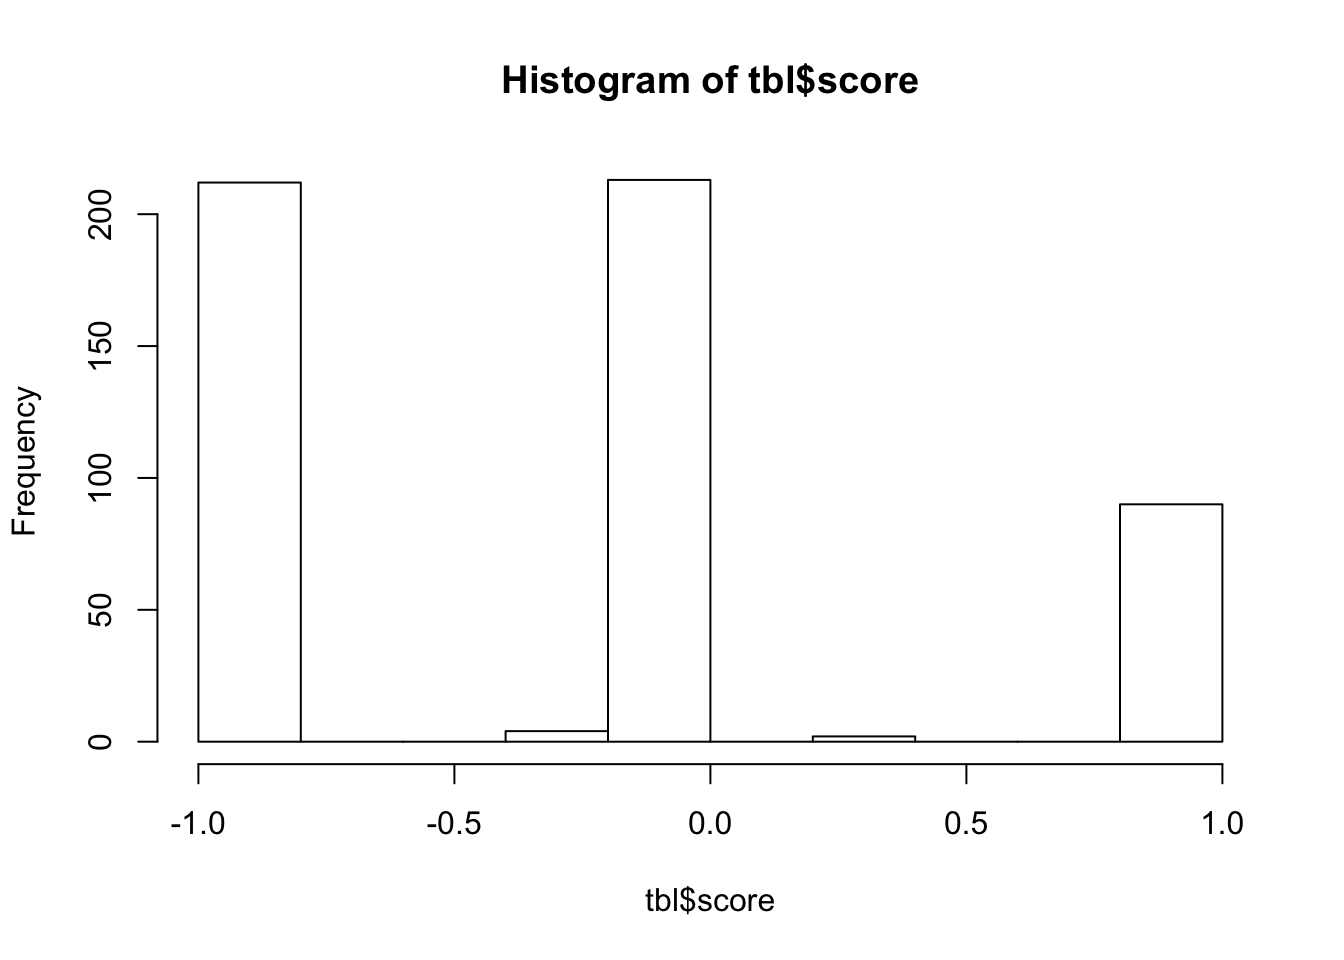
\includegraphics{MEDS-demo_files/figure-latex/unnamed-chunk-10-1.pdf}

\begin{Shaded}
\begin{Highlighting}[]
\KeywordTok{mean}\NormalTok{(}\KeywordTok{na.omit}\NormalTok{(tbl}\OperatorTok{$}\NormalTok{score))}
\end{Highlighting}
\end{Shaded}

\begin{verbatim}
## [1] -0.2354447
\end{verbatim}

\begin{Shaded}
\begin{Highlighting}[]
\KeywordTok{nrow}\NormalTok{(tbl)}
\end{Highlighting}
\end{Shaded}

\begin{verbatim}
## [1] 607
\end{verbatim}

\hypertarget{test-dataset}{%
\section{Test dataset}\label{test-dataset}}

\href{http://help.sentiment140.com/for-students}{For Academics - Sentiment140 - A Twitter Sentiment Analysis Tool}

\begin{Shaded}
\begin{Highlighting}[]
\NormalTok{test_csv <-}\StringTok{ }\KeywordTok{here}\NormalTok{(}\StringTok{"data/sentiment140_testdata.manual.2009.06.14.csv"}\NormalTok{)}
\NormalTok{test <-}\StringTok{ }\KeywordTok{read_csv}\NormalTok{(}
\NormalTok{  test_csv, }\DataTypeTok{col_names =} \KeywordTok{c}\NormalTok{(}
    \StringTok{"polarity"}\NormalTok{, }\StringTok{"status_id"}\NormalTok{, }\StringTok{"created_at"}\NormalTok{, }\StringTok{"query"}\NormalTok{, }\StringTok{"screen_name"}\NormalTok{, }\StringTok{"text"}\NormalTok{)) }\OperatorTok\StringTok{ }
\StringTok{  }\KeywordTok{mutate}\NormalTok{(}
    \CommentTok{# convert negative 0 -> -1, neutral 2 -> 0, positive 4 -> 1  }
    \DataTypeTok{polarity =} \KeywordTok{recode}\NormalTok{(polarity, }\StringTok{`}\DataTypeTok{0}\StringTok{`}\NormalTok{ =}\StringTok{ }\DecValTok{-1}\NormalTok{, }\StringTok{`}\DataTypeTok{2}\StringTok{`}\NormalTok{ =}\StringTok{ }\DecValTok{0}\NormalTok{, }\StringTok{`}\DataTypeTok{4}\StringTok{`}\NormalTok{ =}\StringTok{ }\DecValTok{1}\NormalTok{))}

\CommentTok{# clean out non-ascii, twitter handles, and urls}
\NormalTok{test <-}\StringTok{ }\NormalTok{test }\OperatorTok\StringTok{ }
\StringTok{  }\KeywordTok{mutate}\NormalTok{(}
    \DataTypeTok{text_clean =}\NormalTok{ text }\OperatorTok\StringTok{ }
\StringTok{      }\KeywordTok{str_replace_all}\NormalTok{(}\StringTok{"[^[:ascii:]]"}\NormalTok{, }\StringTok{"_"}\NormalTok{) }\OperatorTok\StringTok{ }
\StringTok{      }\KeywordTok{tolower}\NormalTok{() }\OperatorTok\StringTok{ }
\StringTok{      }\KeywordTok{str_replace_all}\NormalTok{(}\StringTok{"@[^ ]+"}\NormalTok{, }\StringTok{"_usr_"}\NormalTok{) }\OperatorTok\StringTok{ }
\StringTok{      }\KeywordTok{str_replace_all}\NormalTok{(}\StringTok{"http[^ ]+"}\NormalTok{, }\StringTok{"_url_"}\NormalTok{))}

\CommentTok{# tweets to words}
\NormalTok{words <-}\StringTok{ }\NormalTok{test }\OperatorTok\StringTok{ }
\StringTok{  }\KeywordTok{select}\NormalTok{(status_id, created_at, screen_name, text_clean) }\OperatorTok\StringTok{ }
\StringTok{  }\KeywordTok{unnest_tokens}\NormalTok{(}\DataTypeTok{output =}\NormalTok{ word, }\DataTypeTok{input =}\NormalTok{ text_clean, }\DataTypeTok{token =} \StringTok{"words"}\NormalTok{) }\OperatorTok\StringTok{ }
\StringTok{  }\KeywordTok{anti_join}\NormalTok{(stop_words, }\DataTypeTok{by =} \StringTok{"word"}\NormalTok{) }\OperatorTok\StringTok{ }
\StringTok{  }\KeywordTok{left_join}\NormalTok{(s_b, }\DataTypeTok{by =} \StringTok{"word"}\NormalTok{) }\OperatorTok\StringTok{ }
\StringTok{  }\KeywordTok{left_join}\NormalTok{(}
    \KeywordTok{tribble}\NormalTok{(}
      \OperatorTok{~}\NormalTok{sentiment, }\OperatorTok{~}\NormalTok{score,}
      \StringTok{"positive"}\NormalTok{, }\DecValTok{1}\NormalTok{,}
      \StringTok{"negative"}\NormalTok{, }\DecValTok{-1}\NormalTok{),}
    \DataTypeTok{by =} \StringTok{"sentiment"}\NormalTok{)}

\CommentTok{# tally score per tweet}
\NormalTok{test <-}\StringTok{ }\NormalTok{test }\OperatorTok\StringTok{ }
\StringTok{  }\KeywordTok{left_join}\NormalTok{(}
\NormalTok{    words }\OperatorTok\StringTok{ }
\StringTok{      }\KeywordTok{group_by}\NormalTok{(status_id) }\OperatorTok\StringTok{ }
\StringTok{      }\KeywordTok{summarize}\NormalTok{(}
        \DataTypeTok{score =} \KeywordTok{mean}\NormalTok{(score, }\DataTypeTok{na.rm =}\NormalTok{ T)),}
    \DataTypeTok{by =} \StringTok{"status_id"}\NormalTok{)}

\KeywordTok{hist}\NormalTok{(test}\OperatorTok{$}\NormalTok{score)}
\end{Highlighting}
\end{Shaded}

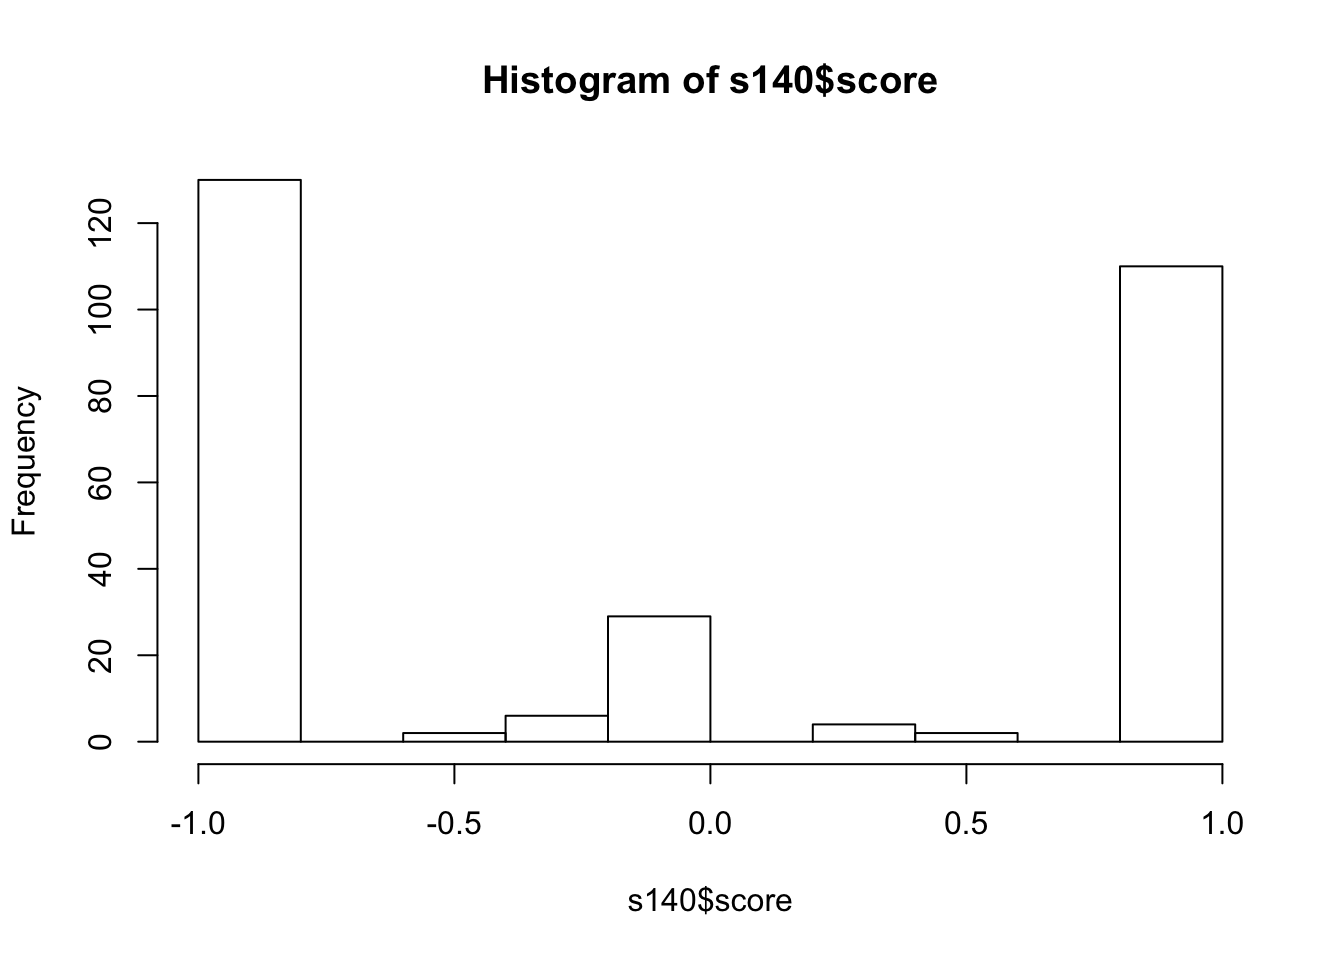
\includegraphics{MEDS-demo_files/figure-latex/unnamed-chunk-11-1.pdf}

\begin{Shaded}
\begin{Highlighting}[]
\KeywordTok{nrow}\NormalTok{(test)}
\end{Highlighting}
\end{Shaded}

\begin{verbatim}
## [1] 498
\end{verbatim}

\begin{Shaded}
\begin{Highlighting}[]
\KeywordTok{mean}\NormalTok{(}\KeywordTok{na.omit}\NormalTok{(test}\OperatorTok{$}\NormalTok{score))}
\end{Highlighting}
\end{Shaded}

\begin{verbatim}
## [1] -0.07255595
\end{verbatim}

\hypertarget{introducing-tensorflow}{%
\section{Introducing TensorFlow}\label{introducing-tensorflow}}

\href{https://blogs.rstudio.com/ai/posts/2019-12-18-tfhub-0.7.0/}{RStudio AI Blog: tfhub: R interface to TensorFlow Hub}

You need to install these Python packages once:

\begin{Shaded}
\begin{Highlighting}[]
\NormalTok{tensorflow}\OperatorTok{::}\KeywordTok{install_tensorflow}\NormalTok{()}
\NormalTok{keras}\OperatorTok{::}\KeywordTok{install_keras}\NormalTok{()}
\NormalTok{tfhub}\OperatorTok{::}\KeywordTok{install_tfhub}\NormalTok{()}
\NormalTok{tfds}\OperatorTok{::}\KeywordTok{install_tfds}\NormalTok{()}
\NormalTok{reticulate}\OperatorTok{::}\KeywordTok{py_config}\NormalTok{()}
\end{Highlighting}
\end{Shaded}

\begin{Shaded}
\begin{Highlighting}[]
\KeywordTok{library}\NormalTok{(tfhub)}
\KeywordTok{library}\NormalTok{(keras)}

\NormalTok{layer_mobilenet <-}\StringTok{ }\KeywordTok{layer_hub}\NormalTok{(}
  \DataTypeTok{handle =} \StringTok{"https://tfhub.dev/google/tf2-preview/mobilenet_v2/classification/4"}\NormalTok{)}

\NormalTok{input  <-}\StringTok{ }\KeywordTok{layer_input}\NormalTok{(}\DataTypeTok{shape =} \KeywordTok{c}\NormalTok{(}\DecValTok{224}\NormalTok{, }\DecValTok{224}\NormalTok{, }\DecValTok{3}\NormalTok{))}
\NormalTok{output <-}\StringTok{ }\KeywordTok{layer_mobilenet}\NormalTok{(input)}
\NormalTok{model  <-}\StringTok{ }\KeywordTok{keras_model}\NormalTok{(input, output)}
\KeywordTok{summary}\NormalTok{(model)}
\end{Highlighting}
\end{Shaded}

The \texttt{layer\_hub()} function above however kept throwing errors like this:

\begin{verbatim}
Error in py_call_impl(callable, dots$args, dots$keywords) : 
  OSError: SavedModel file does not exist at: /var/folders/2r/grqvdjfn04361tzk8mh60st40000gn/T/tfhub_modules/426589ad685896ab7954855255a52db3442cb38d/{saved_model.pbtxt|saved_model.pb}
\end{verbatim}

There's a lot of Python and R communication that can get easily confused between versions. So let's switch to a clean installation by using Docker. \href{https://docs.docker.com/get-docker/}{Install Docker} if you don't already have it.

Then per \href{https://hub.docker.com/r/rocker/tensorflow}{rocker/tensorflow - Docker Hub} run the following to get a clean RStudio instance with all the TensorFlow and Python dependencies properly installed:

\begin{Shaded}
\begin{Highlighting}[]
\ExtensionTok{docker}\NormalTok{ run -e PASSWORD=mu -p 8787:8787 rocker/ml}
\end{Highlighting}
\end{Shaded}

\begin{Shaded}
\begin{Highlighting}[]
\NormalTok{img <-}\StringTok{ }\KeywordTok{image_load}\NormalTok{(}\StringTok{"data/grace-hopper.jpg"}\NormalTok{, }\DataTypeTok{target_size =} \KeywordTok{c}\NormalTok{(}\DecValTok{224}\NormalTok{,}\DecValTok{224}\NormalTok{)) }\OperatorTok\StringTok{ }
\KeywordTok{image_to_array}\NormalTok{()}
\NormalTok{img <-}\StringTok{ }\NormalTok{img}\OperatorTok{/}\DecValTok{255}
\KeywordTok{dim}\NormalTok{(img) <-}\StringTok{ }\KeywordTok{c}\NormalTok{(}\DecValTok{1}\NormalTok{, }\KeywordTok{dim}\NormalTok{(img))}
\NormalTok{pred <-}\StringTok{ }\KeywordTok{predict}\NormalTok{(model, img)}
\KeywordTok{imagenet_decode_predictions}\NormalTok{(pred[,}\OperatorTok{-}\DecValTok{1}\NormalTok{,}\DataTypeTok{drop=}\OtherTok{FALSE}\NormalTok{])[[}\DecValTok{1}\NormalTok{]]}
\end{Highlighting}
\end{Shaded}

\bibliography{style/zotero\_meds-demo.bib}

\end{document}
